%Einleitungstext zum Modul
\section{Klassen}
\graphicspath{{./img/logger/}}
%Bild der Klasse aus dem Klassendiagramm (nur die Klasse jeweils)
%Dokumentation zur Klasse, öffentlichen Methoden und Konstruktor sowie:
%Signal und Slots als Methoden mit Rückgabewert Sigal bzw Slot (zur kenntlichkeit) 
\subsubsection{CLogInit}\label{Logger: CLogInit}
%\includegraphics[scale=1, resolution=100]{}\\
Initialisierungsklasse für den Logger erzeugt bei Objekterzeugung die  otextstream-Objekte und gibt über die Schnittstellen Objektreferenzen weiter. 
\beginAttributes
\newAttribute{private infostream}{Objekt Referenz auf das otextstream-Objekt zum loggen der Infonachrichten}
\newAttribute{private errorstream}{Objekt Referenz auf das otextstream-Objekt zum loggen der Errornachrichten}
\newAttribute{private debugstream}{Objekt Referenz auf das otextstream-Objekt zum loggen der Debugnachrichten}
\newAttribute{private warningstream}{Objekt Referenz auf das otextstream-Objekt zum loggen der Warningnachrichten}
\closeMembers
\beginMembers
\newMember{{getInfostream}}{void}{otextstream}{Gibt eine Objektreferenz auf das Infostream Objekt zurück}
\newMember{{getErrorstream}}{void}{otextstream}{Gibt eine Objektreferenz auf das Errorstream Objekt zurück}
\newMember{{getDebugstream}}{void}{otextstream}{Gibt eine Objektreferenz auf das Debugstream Objekt zurück}
\newMember{{getWarningstream}}{void}{otextstream}{Gibt eine Objektreferenz auf das Waningstream Objekt zurück}
\closeMembers





\subsection{CLogController}\label{Logger: CLogController}
%\includegraphics[scale=1, resolution=100]{}\\
Überprüft die otextstream-Objekte und stellt das Bindeglied zwischen der QSLog Biblothek, GUI und otextstream Objekte da. 
\beginMembers
\newMember{{refreshLog}}{void}{void}{Überprüft die otextstreamobjekte auf neue Nachrichten ud gibt diese an die GUI(per Signal) an den QSLogger und an die History weiter}
\newMember{{setLog}}{dest : QString}{void}{setzt den Datenpfad für ein Log auf den momentanen Ergebnissordner. Muss beim Start des Algorithmendurchlaufs gesetzt werden}
\newMember{{closeLog}}{void}{void}{schließt das aktuelle Log ab. Muss nach Ende des Algorithmendurchlaufs ausgeführt werden}
\closeMembers
\beginSignals
\newSignal{newLogMessage}{message: QString, time: QString}{Wird aufgerufen, wenn eine neue Lognachricht vorhanden ist}
\closeMembers
\section{Pakete}
%Einteilung der Teilmodule in Pakete 
\subsection{Paket 1}
%Bild des Pakets mit vereinfachter Klassendarstellung
%Begründung / Dokumentation / Erklärung zum Paket
\subsection{Paket 2}
%....
\section{Entwurfsmuster}
% verwendete Entwurfsmuster aufzählen erklären etc mit verinfachtem Diagramm (Klassen ohne Inhalt nur die Namen)

\section{Klassendiagramm}
% Klassendiagramm des Moduls
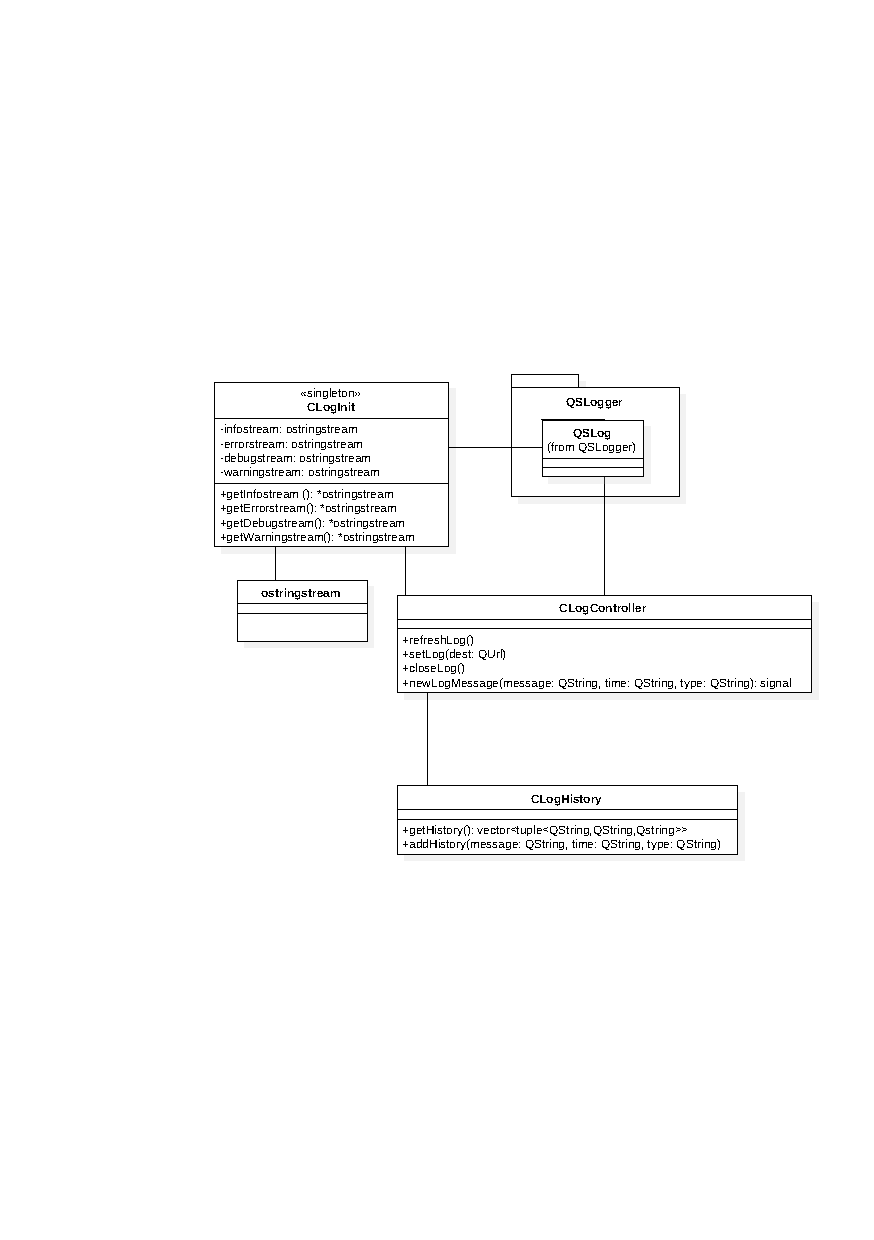
\includegraphics[width=\linewidth]{Klassendiagramm}
%Bitte jeweils kleine Einleitungstexte usw in Unterkapitel gerne auch in Textform Erklärungen zufügen und auf mögliche erweiterungen durch die kann Kriterien eingehen soweit nötig !